\chapter{Experimental Results}
For building a classifier a dataset of 2500 frames is generated from BDD100k Dataset \cite{berkeley} from Berkeley University. From these frames,  500 frames are chosen randomly in which all the vehicles are normal or safe with respect to host  vehicle and 500 frames are chosen such that some vehicles in these frames are abnormal or dangerous with respect to host vehicle. 

\section{Results}

The following figure 7.1 shows the object detection step's output using YOLO algorithm.

\begin{figure}[h]
\begin{center}
    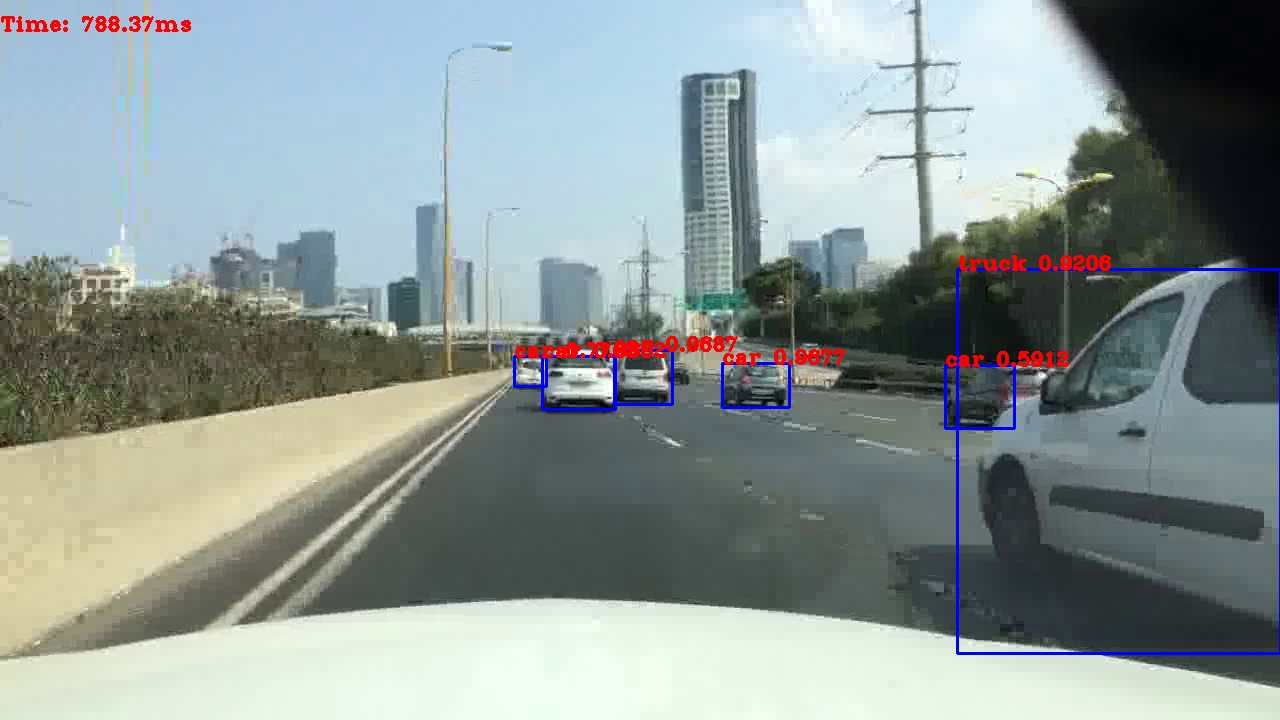
\includegraphics[scale=.25]{yolo.jpeg}
    \caption{Object detecion using YOLO}
\end{center}
\end{figure}

Following figure 7.2 shows the optical flow vector for every pixel of each bounding box using optical flow analysis and figure 7.3 shows the aggregated optical flow vector or motion vector for each vehicle. Aggregation is done by simple averaging of all the optical flow vectors in each bounding box.

\begin{figure}[h]
\begin{center}
    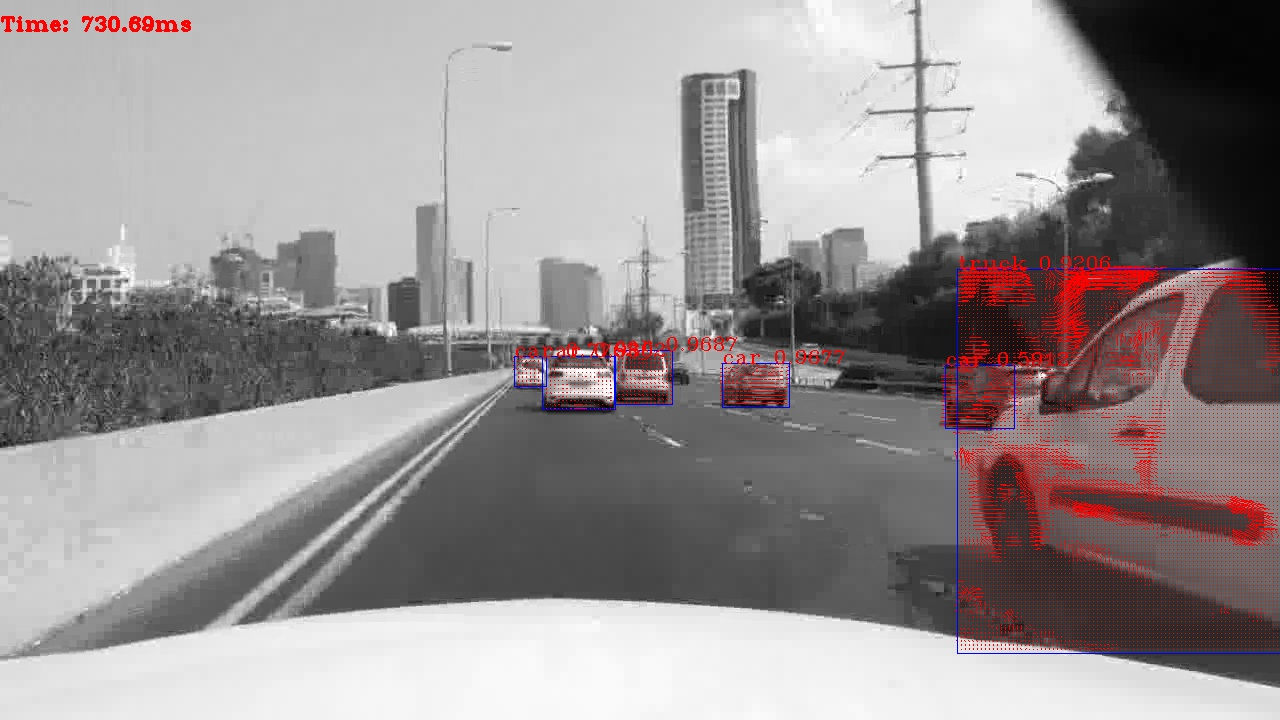
\includegraphics[scale=.25]{optical.jpeg}
    \caption{Optical flow vectors for each pixel in a bounding box}
\end{center}
\end{figure}

\begin{figure}[h]
\begin{center}
    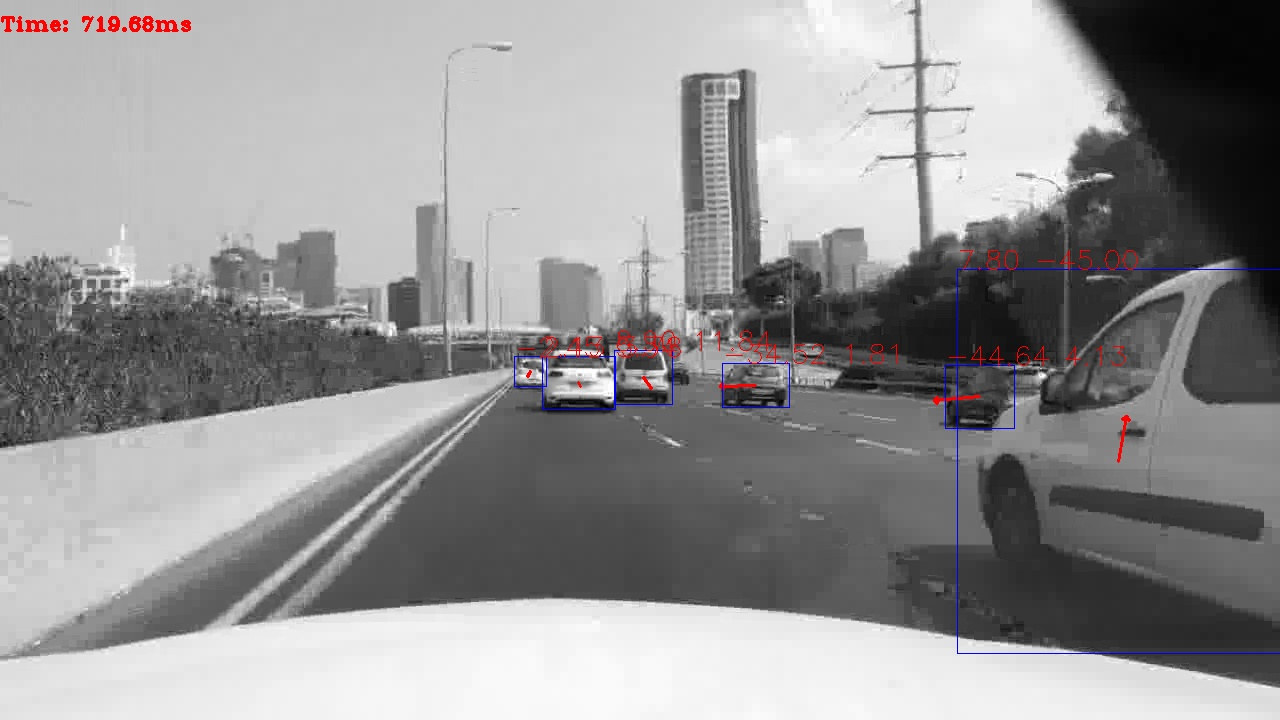
\includegraphics[scale=.25]{motion.jpeg}
    \caption{Aggregated optical flow vectors for each vehicle}
\end{center}
\end{figure}

Using these 1000 chosen frames raw motion vectors are generated. These motion vectors are labelled as abnormal and normal manually. Each row motion vector is represented by four value which are x, y, x+dx, y+dy where (x,y) is tail of vector and (x+dx, y+dy) is head of vectors. All these four values are with relative to host vehicle. Following figure 7.4 visualizes these motion vectors.

\begin{figure}[h]
\begin{center}
    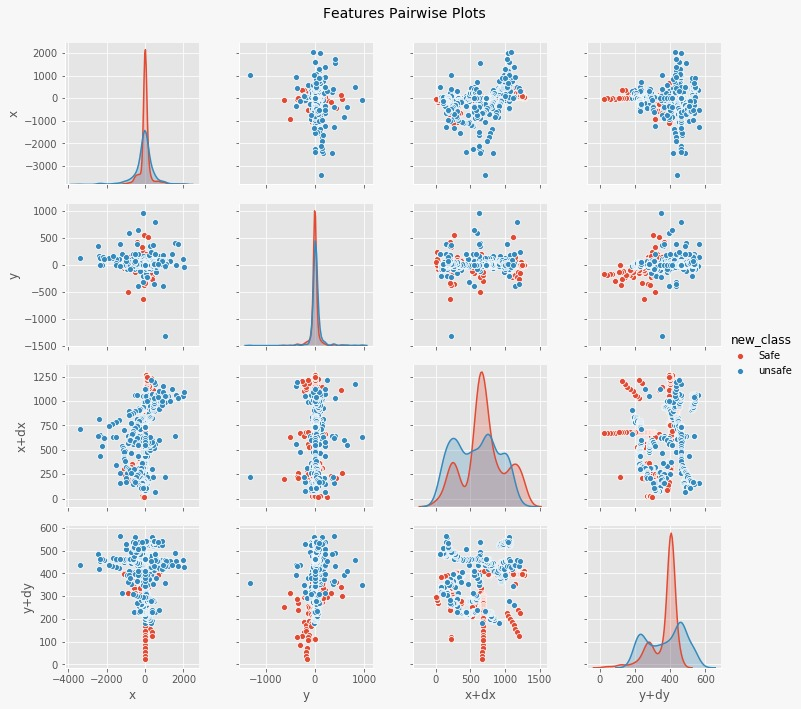
\includegraphics[scale=.45]{pairwise_plot.jpeg}
    \caption{Pairwise scatter plot for visualization of data with respect to each variable}
\end{center}
\end{figure}

Using this dataset of motion vectors,  support vector machine classifier is trained. After training when it is tested on unseen data during training it gives accuracy of 93.57\%. The following figure 7.5  shows the confusion matrix which is result of training of SVM classifier. 

\begin{figure}[H]
    \centering
    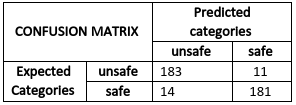
\includegraphics{confusionmtrix.png}
        \caption {Confusion Matrix of test results} \\

\end{figure}



In the figure 7.4 and 7.5, class unsafe denotes abnormal behaviour of vehicles and safe denotes normal behaviour of vehicles with respect to host vehicle.

Further the accuracy of this model is somewhat dependent on dataset. The dataset used in this experimentation is generated manually from standard videos. So if a more good generalised dataset is used then accuracy can still be improved.



\section{Conclusion}
Proposed algorithm is able to solve the problem of abnormal vehicle detection in the surroundings of host vehicle in real time with a good and reliable accuracy of 93.57\%. A model is created which is composed of three different units namely vehicle detection unit, motion analysis unit, classification unit. Job of vehicle detection unit is to detect and localize of vehicles. Motion analysis unit performs motion analysis and generate motion information for moving vehicles. Classification unit performs classification of vehicles into abnormal and normal classes and hence a warning signal is sent to driver.

